\section{Raytracing}
 
\begin{figure}[H]
    \centering
    
\includegraphics[height=0.7\textwidth]{images/mouille.jpg}
    \caption{Ein mit Povray gerendertes Bild aus dem Jahre 2000.}
    \label{fig:povray}
\end{figure}


 \begin{figure}[H]
    \centering
    
\includegraphics[height=0.5\textwidth]{images/vray.png}
    \caption{Ein mit VRay gerendertes Bild aus dem Jahre 2015.}
    \label{fig:cray}
\end{figure}


 \begin{figure}[H]
    \centering
    
\includegraphics[height=0.5\textwidth]{images/freestyle.jpg}
    \caption{Ein nicht photorealistisches Rendering in Blender aus dem Jahre 2015.}
    \label{fig:cray}
\end{figure}


 \begin{figure}[H]
    \centering
    
\includegraphics[height=0.5\textwidth]{images/pixar.jpg}
    \caption{Ein nicht photorealistisches Rendering mit Pixar's renderman aus dem Jahre 2001.}
    \label{fig:cray}
\end{figure}

\subsection{Farbwahrnehmung und Farbmodelle}

\subsection{Globale Beleuchtungsmodelle und Rendergleichung}

\subsubsection{Sphären, Raumwinkel und infinitessimale Flächenstücke}

 \begin{figure}[H]
    \centering
    
\includegraphics[width=0.7\textwidth]{images/solidangle.png}
    \caption{Raumwinkel}
    \label{fig:cray}
\end{figure}

\subsubsection{Photometrie}

Die Radiantenergie $Q$ ist die Lichtenergie (Strahlungsleistung). Sie wird durch einen Strom von Photonen erzeugt. Die Energie eines Photons ist 
durch $E=h \cdot f$ geben, wobei $h$ das konstante Planksche Wirkungsquantum und $f$ die Frequenz der Welle ist (Welle-Teilchen Dualismus).  
Die Ableitung nach der Zeit
\begin{align}
\phi := \frac{\partial Q}{\partial t}
\end{align}
wird als Radiant Flux oder Strahlungsleistung bezeichnet. Die Einheit ist Watt (W).
Diese  beschreibt den Energiefluss, beziehungsweise den Energie-Eintritt und Energie-Austritt.

 \begin{figure}[H]
    \centering
    \includegraphics[height=0.5\textwidth]{images/infrared_dog.jpg}
    \caption{Strahlungsleistung an verschiedenen Punkten der Oberfläche}
    \label{fig:cray}
\end{figure}



Das photometrische Grundgesetzt beschreibt die Strahlung, die von einem infintesimalen Flächenelement auf ein anderes infinitesimales Flächenelement 
übertragen wird.  
 \begin{figure}[H]
    \centering
    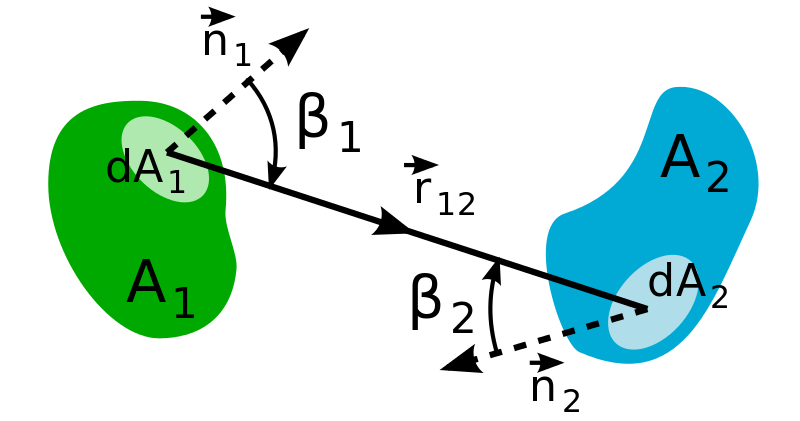
\includegraphics[width=0.7\textwidth]{images/Fotometrisches_Grundgesetz_Schema.png}
    \caption{Fotometrisches Grundgesetz}
    \label{fig:cray}
\end{figure}

\begin{align}
d^2 \phi = L\cdot \cos(\beta_1) \cdot dA_1 \cdot d \omega_2 = \frac{1}{r_{12}^2}  \cdot L \cdot \cos(\beta_1) \cdot \cos(\beta_2) \cdot dA_1 \cdot d \omega_2
\end{align}
Die Radiance $L(x, \omega)$ ist  der Radiant Flux in einem infinitesimal dünnen Strahl vom Punkt $x$ in Richtung $\omega$ und ist 
\begin{align}
L(x, \omega) := \frac{d^2 \phi}{\cos(\theta) \cdot dA \cdot d\omega} 
\end{align}
wobei $\theta$ der Winkel zwischen der Flächennormale am Punkt $x$ und der Richtung $\omega$ ist.
Die Radiance ist also der Radiant Flux pro infinitesimale Flächeneinheit $\cos(\theta) dA$ und pro  Raumwinkel $d \omega$.
Die Einheit ist $\frac{W}{m^2\cdot sr}$ (Watt ($W$) pro Quadratmeter ($m^2$) und pro Steradiant ($sr$)). 
Eine Objekt, dessen Stahldichte für alle Punkte und Richtungen konstant ist, also
$L(x, \omega) = c$  für alle $x \in O$ und $\omega \in S^2$, bezeichnet man auch als Lambertschen Strahler. 

Mit $L_i, L_o,Lr,L_e$ bezeichnet man entsprechend den eintreffende, ausgehende, reflektierte beziehungsweise emittierte Radiance.



Die sogenannte bidirektionale Reflektanzverteilungsfunktion (engl. Bidirectional Reflectance Distribution Function, BRDF)
ist eine Funktion $f_r (x, \omega_i, \omega_r)$, die das Reflexionsverhalten der Oberfläche eines Materials beschreibt. 
Sie hat als Eingabe die ausgehende Richtung $\omega_r$ und die eingehende Richtung  $\omega_i$ am Punkt $x$. 
Sie  liefert den Quotienten aus Strahlungsdichte und Bestrahlungsstärke für die ausgehende Richtung $\omega_r$ und die eingehende Richtung  $\omega_i$ am Punkt $x$.
Sie gibt somit die Abhängigkeit des reflektierten Lichts von der einfallenden Lichtstärke an: 
\begin{align}
dL_r = f_r(x, \omega_i, \omega_r) dE =   f_r(x, \omega_i, \omega_r)  \cdot  L_i(x,\omega_i) \cdot  \cos(\theta_i) d \omega_i\\
L_r(x, \omega_r) = \int_{S^2} dL_r =    \int_{S^2}f_r (x, \omega_i, \omega_r) \cdot L_i(x, \omega_i) \cdot  \cos(\theta_i) d\omega_i
\end{align}
Letztere Gleichung wird auch Reflectance-Gleichung genannt.
 \begin{figure}[H]
    \centering
    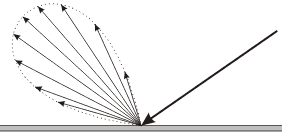
\includegraphics[width=0.6\textwidth]{images/brdf2.png}
    \caption{BRDF Funktion}
    \label{fig:raytracin_brdf}
\end{figure}


 
\subsubsection{Die Rendergleichung (Erste und zweite Form)}

Durch Hinzunahme des von dem Oberflächenpunkt emittierten Lichtes $L_e(x, \omega_o)$ zu dem   an diesem Punkt reflektiert Lichtes erhalten wir die sogenannte Renderingleichung 
\begin{align}
L_o(x, \omega_o) = L_e(x, \omega_o)  + \displaystyle \int_{S^2}f_r (x, \omega_i, \omega_0) \cdot L_i(x, \omega_i)  \cdot  \cos(\theta_i) d\omega_i \; .
\end{align}

Dieses Integral kann durch eine Integraltransformation in eine handlichere Form gebracht werden. Insbesondere die Berechnung der Einfallenden Irradiance  $L_i(x, \omega_i)$  ist in keinster weise offensichtlich. 



Durch die Beziehung $d_omega_i = $

\subsection{Raycasting}
\subsubsection{"Klassisches" Raytracing}
\subsubsection{Radiocity Verfahren}
\subsubsection{Monte Carlo Integration und Pathtracing}
\subsubsection{Raymarching}
\subsection{Klassifikation der Verfahren}

\subsection{Datenstrukturen für Bereichsabfragen}


\subsection{Labor}
\subsubsection{Blender}
\subsubsection{Echtzeitfähiges Raymarching in WebGL}
